\chapter{The \nova~Experiment}
\label{ch:nova}

The \nova~experiment, or the NuMI Off-Axis $\nue$ Appearance experiment, is a long baseline, two detector, neutrino oscillation experiment designed to measure $\numu$ to $\nue$ appearance from the Fermilab NuMI beam. The two functionally identical \nova~detectors are situated $14.6\unit{mrad}$ off-axis of the beam center, with its Near Detector (ND) located approximately $1\unit{km}$ downstream of the beam target source and its Far Detector (FD) located $810\unit{km}$ from the source in Ash River, MN. The main purpose of the ND is to constrain the neutrino beam energy and composition by measuring the beam very close to its source, i.e., before the neutrinos have had a chance to oscillate. The FD then measures the oscillated neutrinos. This chapter describes the NuMI beam and \nova~detectors in more detail.

\section{The NuMI Beam}

The NuMI beam is a $\numu$ beam generated at Fermi National Accelerator Laboratory, or Fermilab, in Batavia, IL, and the source of neutrinos for the \nova~experiment. The neutrino beam is created by accelerating protons to $120\unit{GeV}$, colliding them with a graphite target, and allowing the products to decay to neutrinos.

The NuMI beam originates with the $120\unit{GeV}$ protons, and these are accelerated in the complex shown in figure \ref{fig:FNAL_AC}. First, negatively charged hydrogen atoms are accelerated to $400\unit{MeV}$ in the Linac. These atoms next enter the Booster synchrotron where the electrons are removed and the protons are accelerated to $8\unit{GeV}$. The output of from the booster is $13$ bunches, $12$ which are extracted into the Recycler Ring, each with approximately $4\times10^{12}$ protons. In a procedure called slip stacking, additional bunches are used to double the intensity of each bunch. The first bunches in the Recycler are decelerated slightly while $6$ new bunches enter the ring. As the two sets of bunches have slightly different energies, they slip relative to each other. When two bunches overlap they are captured with a special RF pulse, creating $6$ larger bunches that are extracted into the Main Injector (MI) and accelerated to $120\unit{GeV}$. Finally, these protons are directed to a target for neutrino production. At this point, the 6 bunches, or the spill, total about $5\times10^{13}$ protons. With a cycle time of $1.333\unit{s}$, the NuMI beam reaches $700\unit{kW}$, which is the most powerful beam in the world \cite{ref:TDRNOvA}.
\begin{figure}[htb]
  \centering
  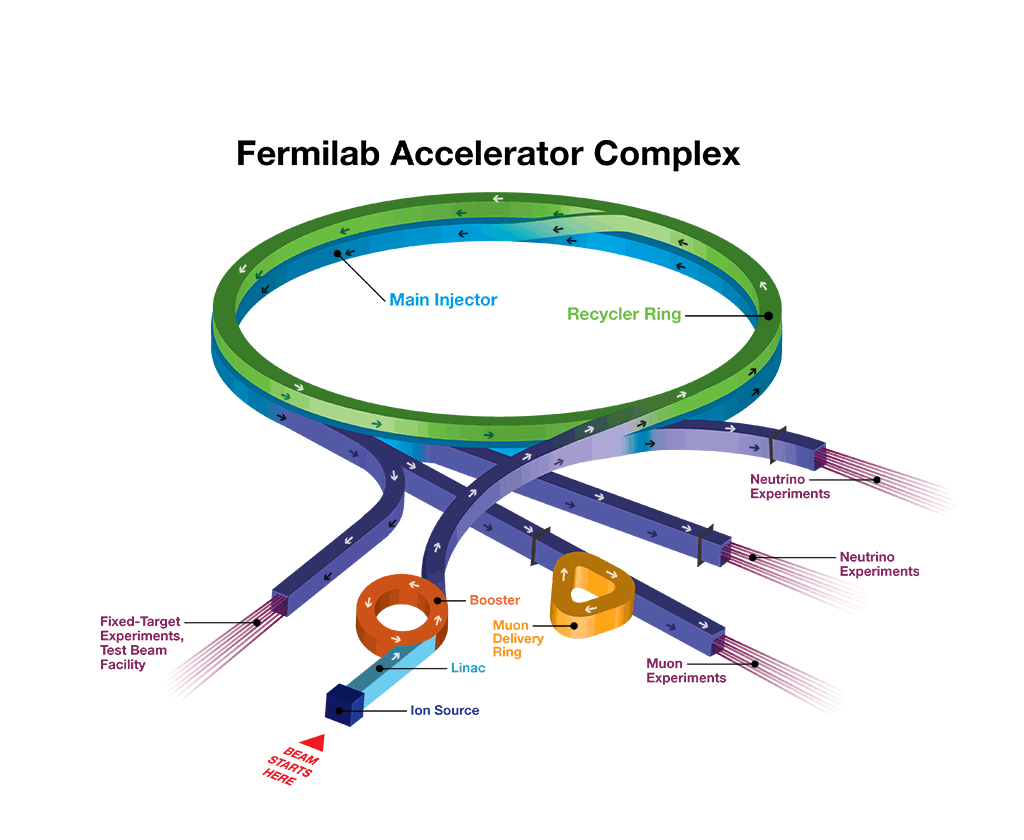
\includegraphics[width=0.75\textwidth]{figures/FNAL_AC.png}
  \caption[Fermilab Accelerator Complex]{Schematic of the Fermilab accelerator complex.}
  \label{fig:FNAL_AC}
\end{figure}

In truth, the above is the design goal of the NuMI beam upgrades. The NuMI beam was originally designed for the MINOS experiment \cite{ref:TDRNuMI}, and it was operating at ${\sim}200\unit{kW}$ with no slip stacking at the time of writing the \nova~Technical Design Report (TDR) in 2007 \cite{ref:TDRNOvA}. Since then, the Fermilab Accelerator Division has been steadily ramping up the beam power, as shown in figure \ref{fig:BeamPower}. At the time of writing of this dissertation, the NuMI beam was in the midst of its 2016 summer shutdown. Before the beam was powered down, it most recently was running stably at about $560\unit{kW}$ with $6{+}4$ slip stacking, or doubling the proton intensity in just $4$ of $6$ bunches \cite{ref:IntensitykW, ref:IntensitySlip}. However, the NuMI beam briefly reached its design goal of $700\unit{kW}$ with full $6{+}6$ slip stacking during a test on June 13, 2016 \cite{ref:Intensity700}.
\begin{figure}[htb]
  \centering
  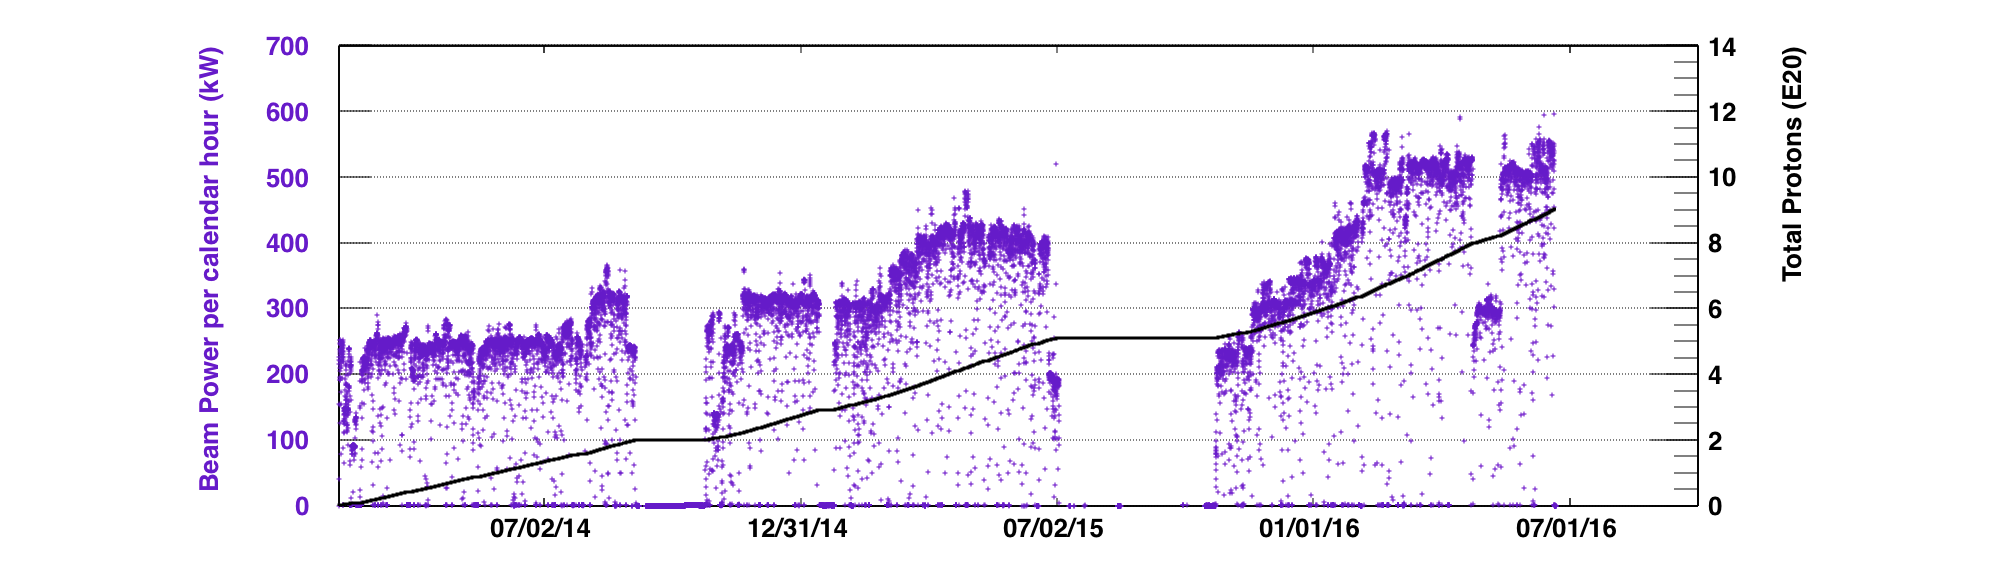
\includegraphics[width=1\textwidth]{figures/BeamPower.png}
  \caption[Beam Power vs Time]{Beam power vs time since \nova~began collecting data. The average beam power is shown as purple points, and the integrated POT is shown in the black curve.}
  \label{fig:BeamPower}
\end{figure}

To generation of the actual neutrino beam begins with the extraction of the $120\unit{GeV}$ protons from the MI into the complex shown as a schematic in figure \ref{fig:FNAL_NuMI}. The protons are directed $3.3^\circ$ downward into the earth so the NuMI beam points directly toward the MINOS FD in Soudan, MN. First the protons collide with atoms inside a long, thin target. The target consists of 47 graphite `fins' that are each $20.0\unit{mm}$ long, $6.4\unit{mm}$ wide, and spaced $0.3\unit{mm}$ apart for a total length of $95.4\unit{cm}$. The beam size at the target is $1\unit{mm} \times 1\unit{mm}$, and the length of the target corresponds to ${\sim}2$ interaction lengths for the protons \cite{ref:TDRNuMI}. \nova~performs its data accounting by summing the protons on target, or POT. The interactions in the target produce a large number of secondary hadrons consisting mainly of charged pions with a smaller contribution of kaons. These particles next pass through two magnetic, parabolic horns. A current of $200\unit{kA}$ is passed through the horns creating a $1/r$ magnetic field that focuses a one sign of the charged particles and defocuses the opposite sign. The current in the horns can be reversed, which allows the NuMI beam to run in either neutrino or antineutrino mode. When positively charged particles are focused, they decay into neutrinos, and similar for negatively charged particles and antineutrinos. Next, the focused charged particles travels through a $675\unit{m}$ long, $1\unit{m}$ radius decay pipe where the hadrons decay into neutrinos and tertiary charged leptons \cite{ref:TDRNOvA}. Finally, everything passes through a hadron monitor and absorber followed by three muon monitors spaced between sections of rock, leaving only the neutrinos to reach the ND hall.
\begin{figure}[htb]
  \centering
  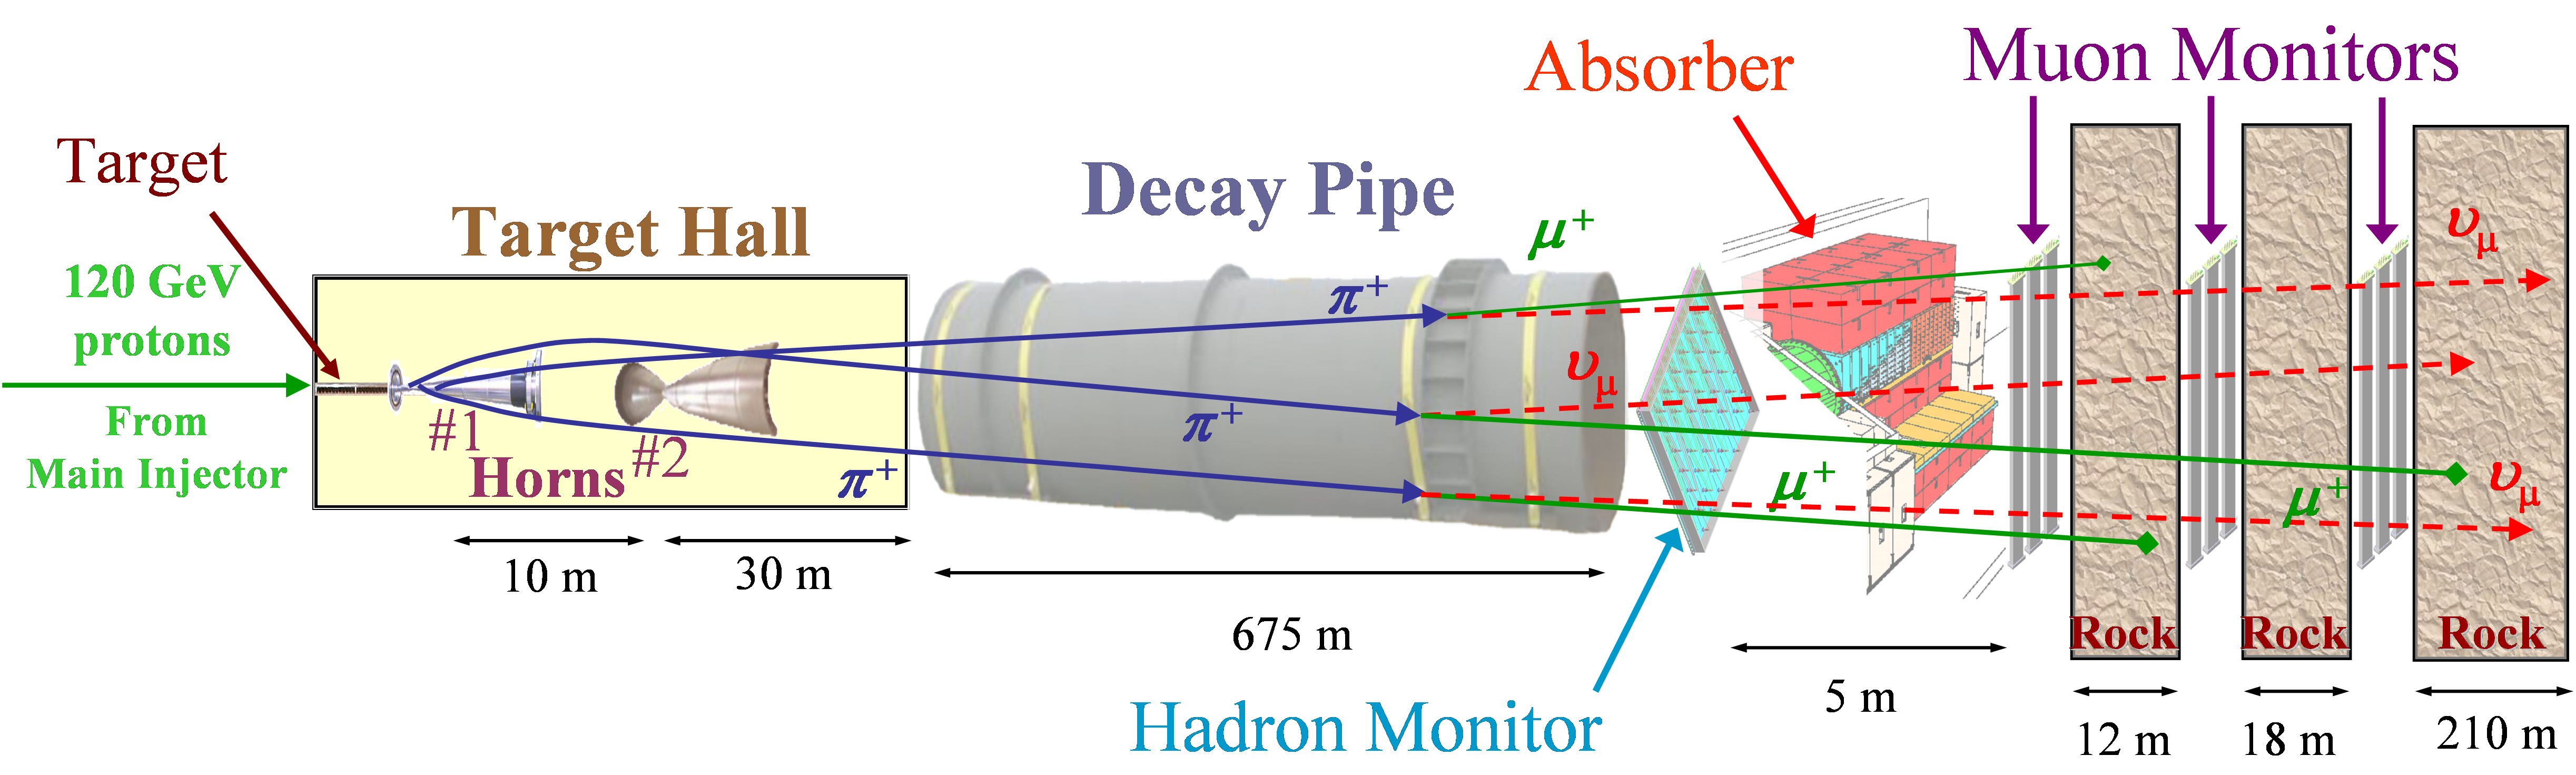
\includegraphics[width=1\textwidth]{figures/FNAL_NuMI.png}
  \caption[NuMI Beam Schematic]{Schematic of the NuMI beam.}
  \label{fig:FNAL_NuMI}
\end{figure}

As a final note for this section, all of the data analyzed in this dissertation was taken during neutrino mode running, so the anti-neutrino mode is not considered further.

\section{Off-Axis Detectors}

The \nova~experiment was designed to have its detectors located $14.6\unit{mrad}$ off-axis from the NuMI beam, and this greatly affects the observed neutrino energy spectrum. The main decay mode for charged pions ($99.98770\%$) and kaons ($63.56\%$) is the two body decay into a muon and muon-neutrino \cite{ref:PDG}. In the center of mass frame of the decaying meson, this is a deterministic, isotropic decay. However, the lab frame is highly boosted resulting in the following neutrino flux and energy spectrum for a detector with cross section area $A$ located a distance $L$ from the decay point.
\beqa
\phi_\nu & = & \left( \frac{2\gamma_m}{ 1 + \gamma^2_m \theta^2 } \right)^2 \frac{A}{4\pi L^2} \label{eq:OffAxisFlux} \\
E_\nu & = & \left(1 - \frac{m^2_\mu}{m^2_m} \right) \frac{E_m}{1 + \gamma^2_m \theta^2} \label{eq:OffAxisE}
\eeqa

\n Above, $\theta$ is the angle between the neutrino and meson, and the subscript $m$ refers to the decaying meson, i.e., $E_m$ is the meson energy, $m_m$ is the meson mass, and $\gamma_m$ is $E_m / m_m$. The effects of an off-axis location is shown in figure \ref{fig:OffAxis}. There are two competing effects that occur. While the flux of neutrinos is drastically reduced, the neutrino energy is highly constrained, with a net result of a very narrow band beam of neutrinos.
\begin{figure}[htb]
  \centering
  \begin{tabular}{c c}
    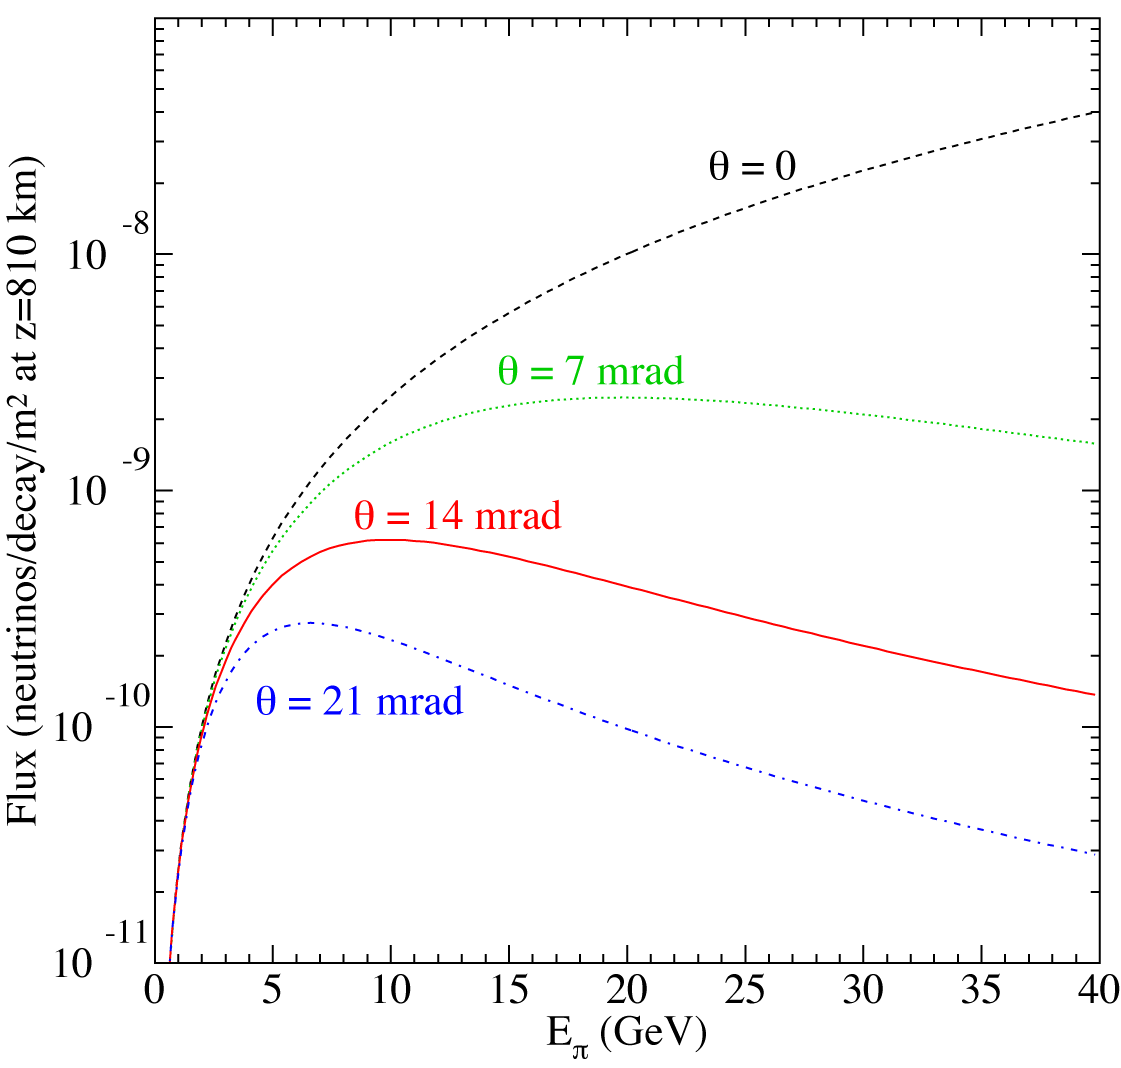
\includegraphics[width=.47\textwidth]{figures/OffAxisFlux.png} &
    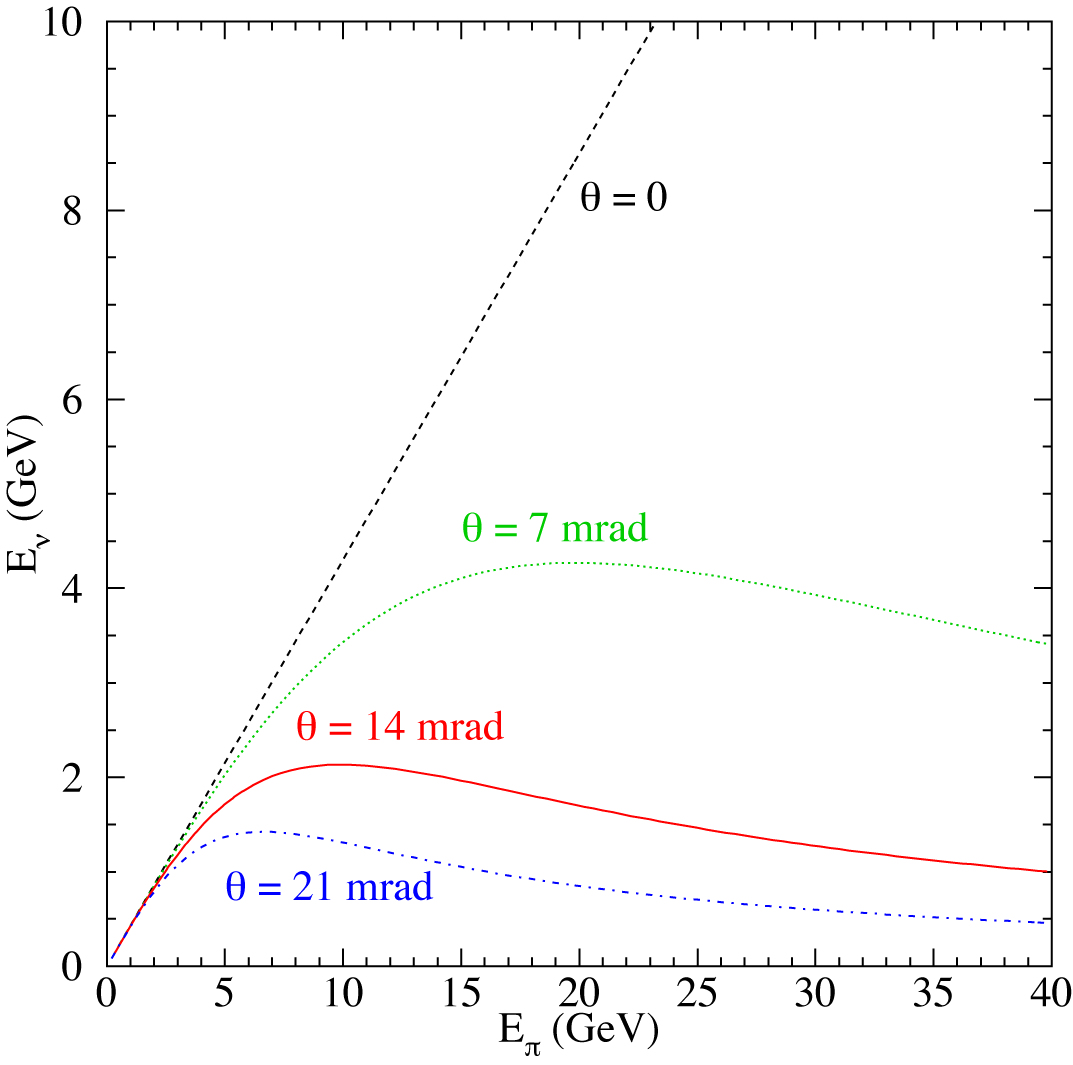
\includegraphics[width=.47\textwidth]{figures/OffAxisE.png} \\
  \end{tabular}
  \caption[Off-Axis Flux and Energy]{The neutrino flux (left) and energy (right) as a function of the decaying pion energy for several different off-axis angles. The on axis values are shown in black, and the red curves show the values for \nova. Plots from \cite{ref:TDRNOvA}}
  \label{fig:OffAxis}
\end{figure}

The narrow energy band result is shown in figure \ref{fig:BeamEComp}, which compares the energy spectrum for several off-axis angles and shows composition of the neutrino beam observed by \nova, both for the FD and without considering oscillations. The small contamination of $\anumu$, $\nue$, and $\anue$ components come from several effects. The focusing horns discussed in the previous section are unable to defocus the most energetic wrong sign mesons, which mostly contributes to the $\anumu$ component through the decay $\pi^- \rightarrow \anumu + \mu^-$. In the decay pipe, some of the muons from pion decay also decay, contributing to both the $\anumu$ and $\nue$ components. While most $K^+$ decay to $\numu$, a small fraction (5.07\% \cite{ref:PDG}) decay via $K^+ \rightarrow \pi^0 + e^+ + \nue$. There is a very small $\anue$ component that is largely due to $K_L$ decay.
\begin{figure}[htb]
  \centering
  \begin{tabular}{c c}
    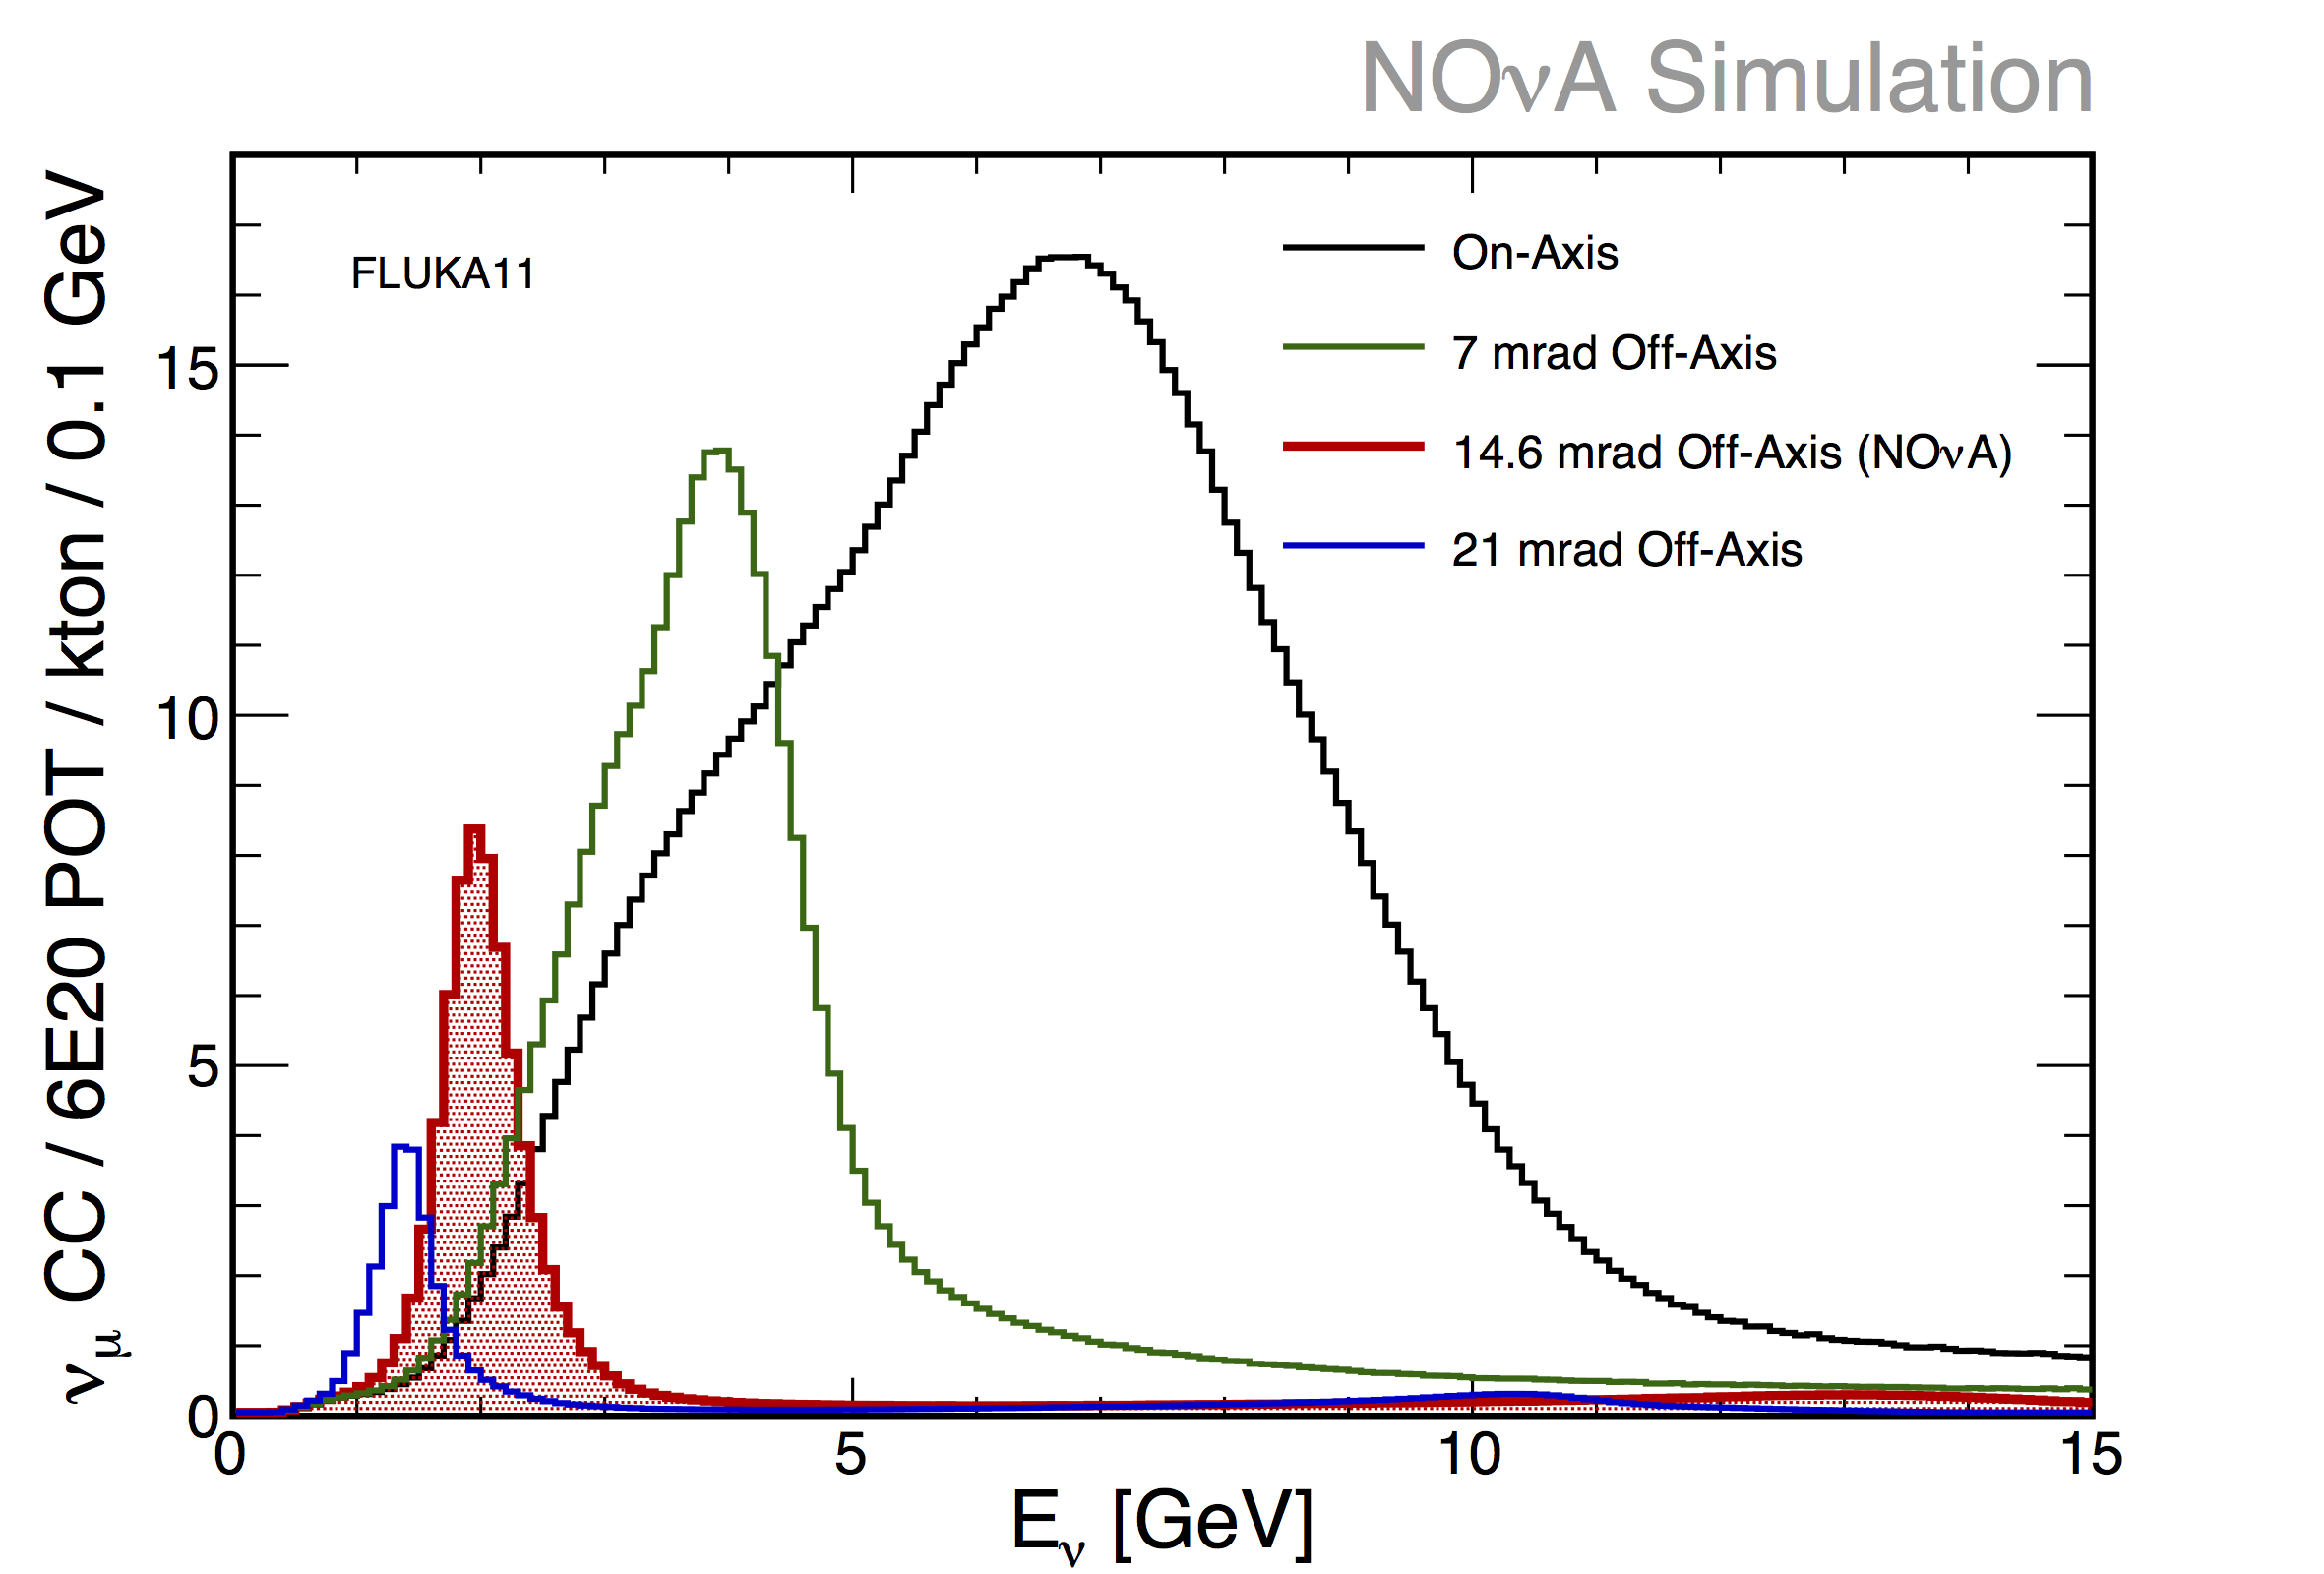
\includegraphics[width=.47\textwidth]{figures/BeamE.png} &
    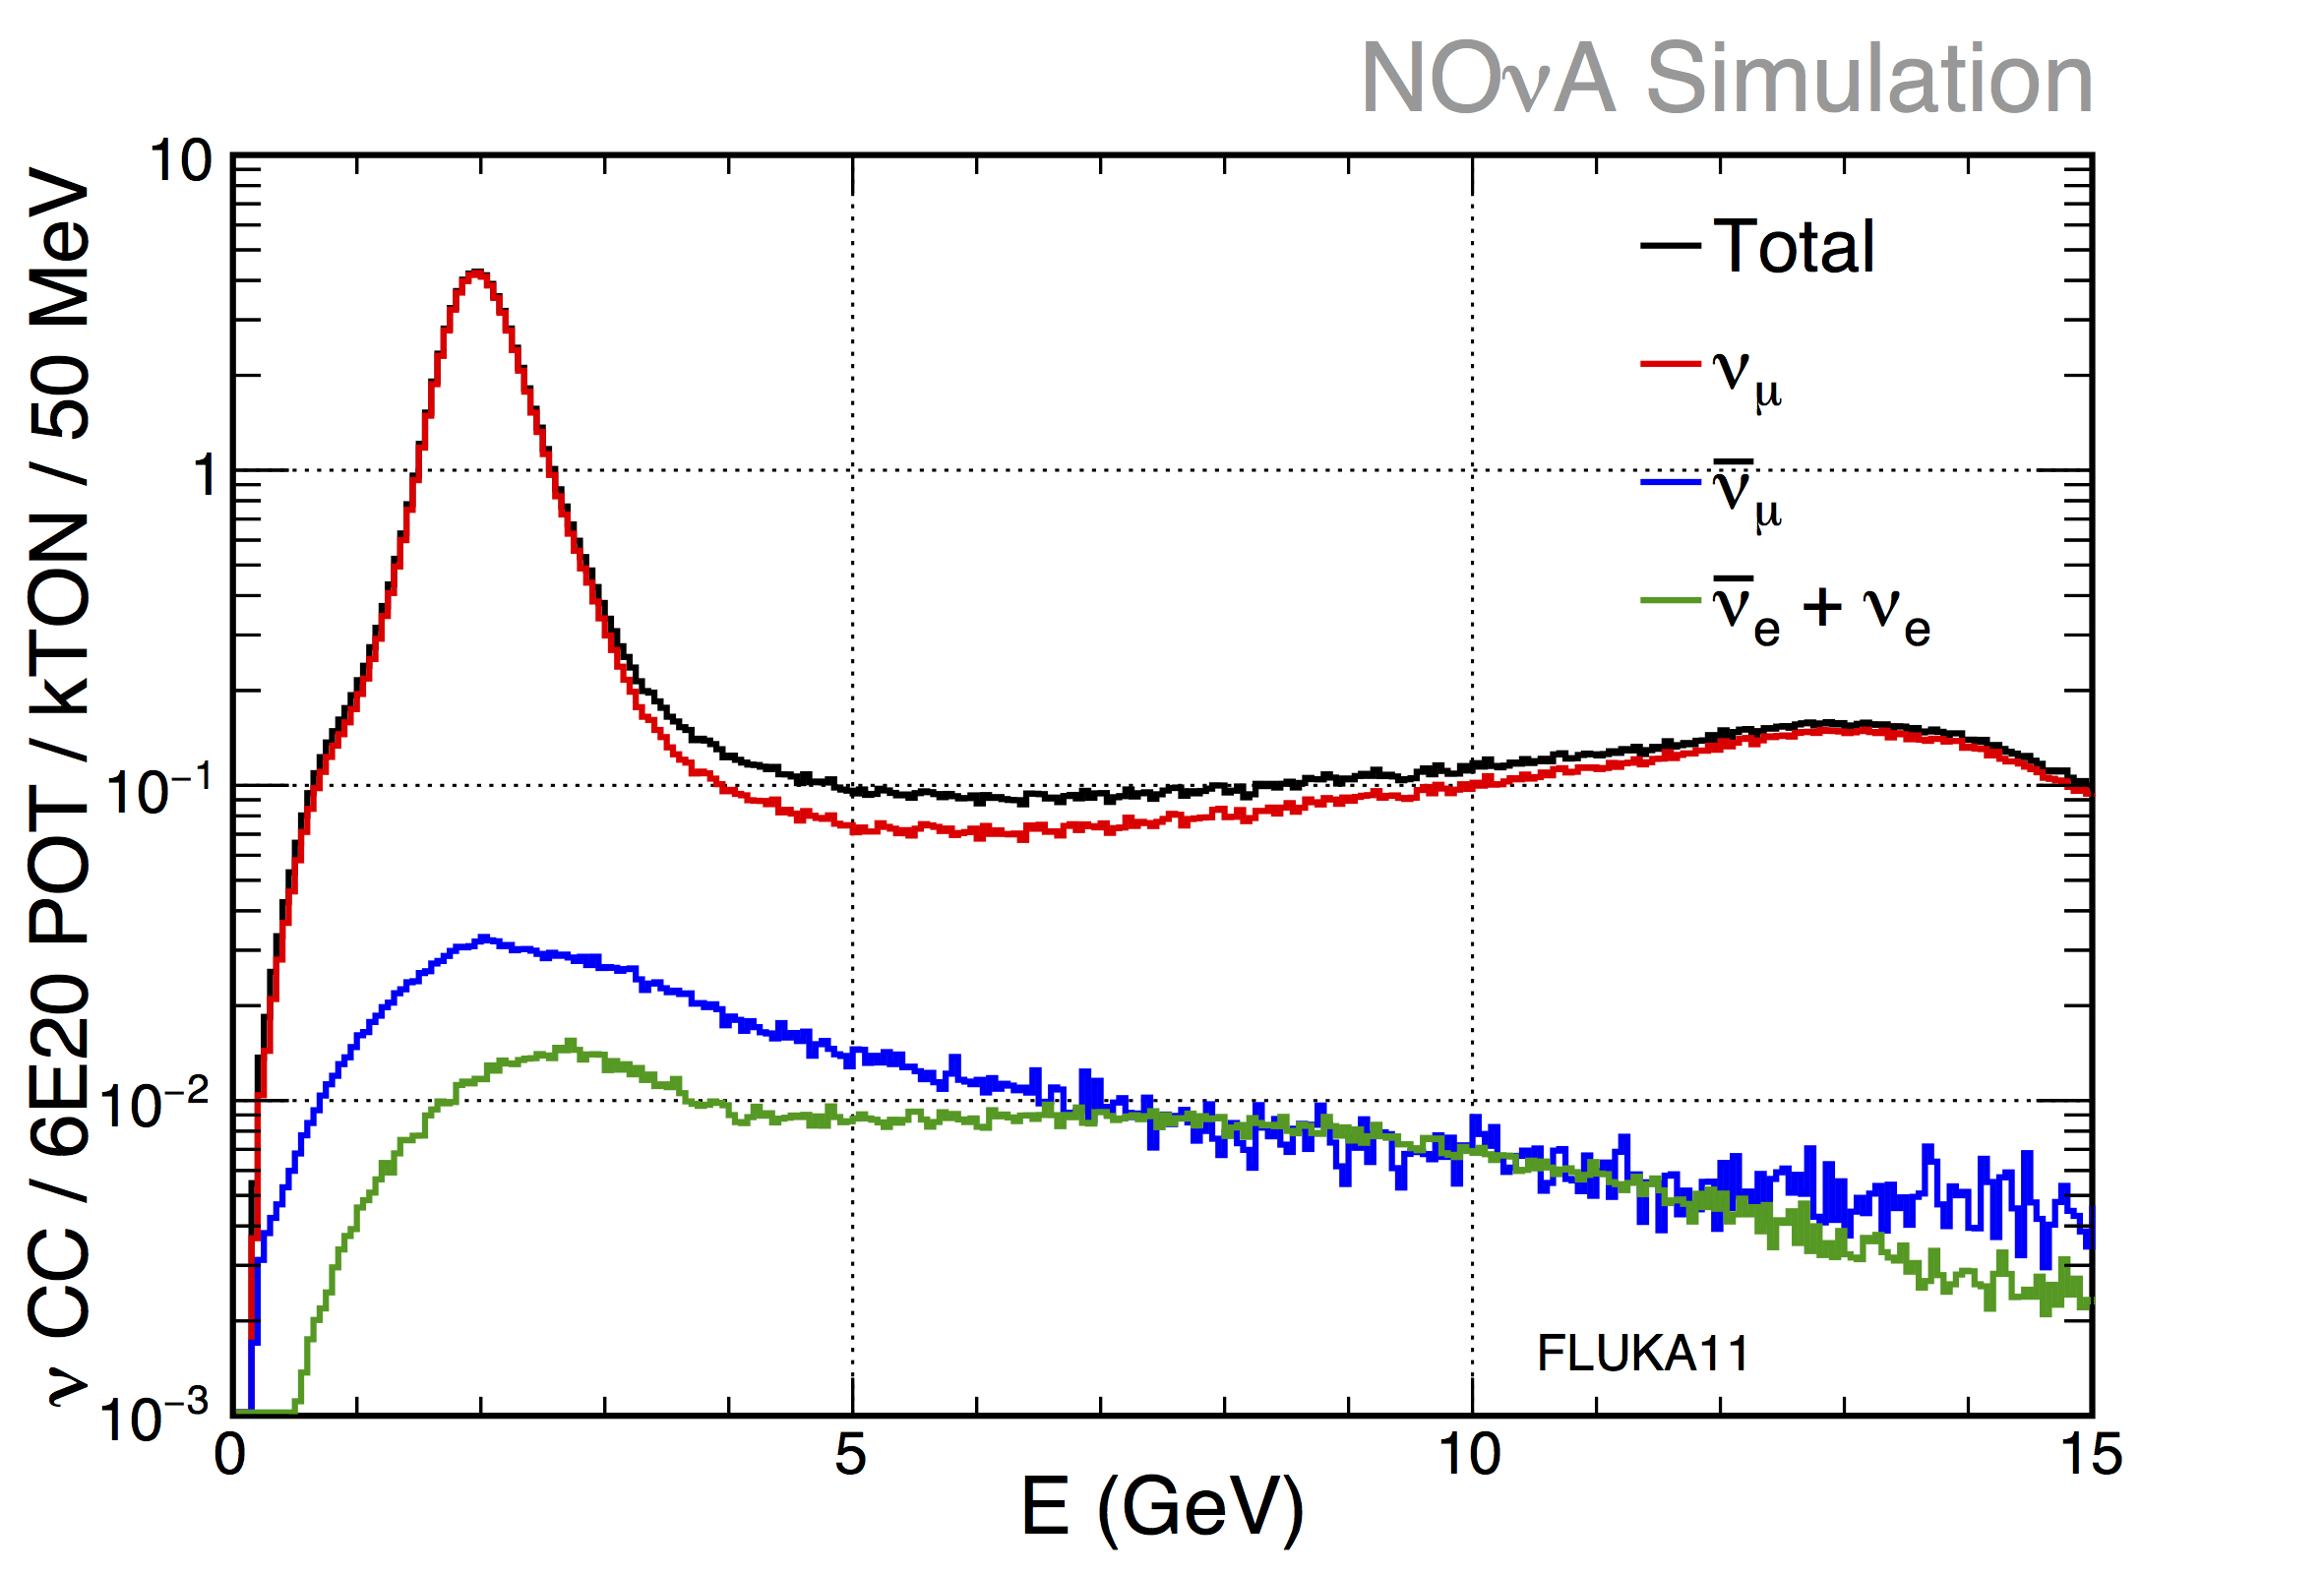
\includegraphics[width=.47\textwidth]{figures/BeamComp.png} \\
  \end{tabular}
  \caption[Beam Energy and Composition]{The neutrino flux (left) and energy (right) as a function of the decaying pion energy for several different off-axis angles. The on axis values are shown in black, and the red curves show the values for \nova.}
  \label{fig:BeamEComp}
\end{figure}

\nova~was designed to be off-axis in an attempt to optimize the amount of observed $\nue$ appearance, as the experiment name would suggest. At the \nova~FD, with $L = 810\unit{km}$, the neutrino energy range observed due to the particular off-axis angle falls right within the first oscillation maximum for $\nue$ appearance. Figure \ref{fig:PMuEFluxXSec} shows the oscillation probability for $\nue$ appearance and the event predictions for the dominant components, both as a function of the true neutrino energy. The narrow band beam and first oscillation peaks match quite well, allowing for the best possible measurement of $\nue$ appearance, one of \nova's two main analyses \cite{ref:NOvAFANuE}. Furthermore, the probability of $\numu$ disappearance (shown only in the event component predictions) highly suppresses the number of expected $\numu$ CC events, allowing for precision measurements of $\numu$ disappearance, the other main \nova~analysis \cite{ref:NOvAFANuMu}.
\begin{figure}[htb]
  \centering
  \begin{tabular}{c c}
    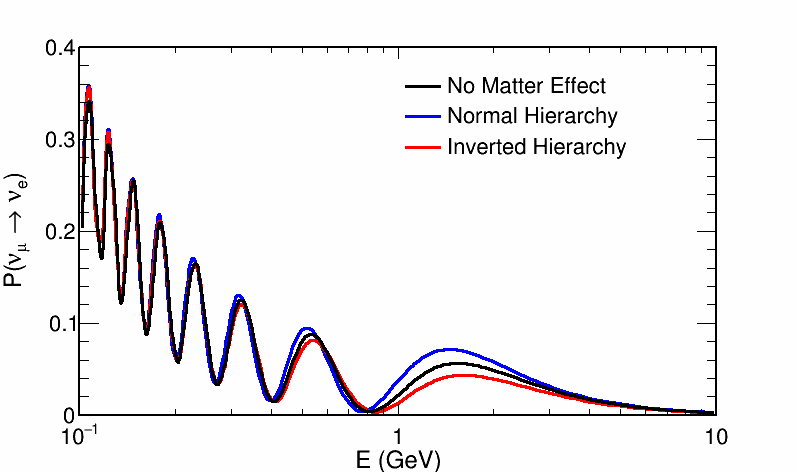
\includegraphics[width=.47\textwidth]{figures/MuE.png} &
    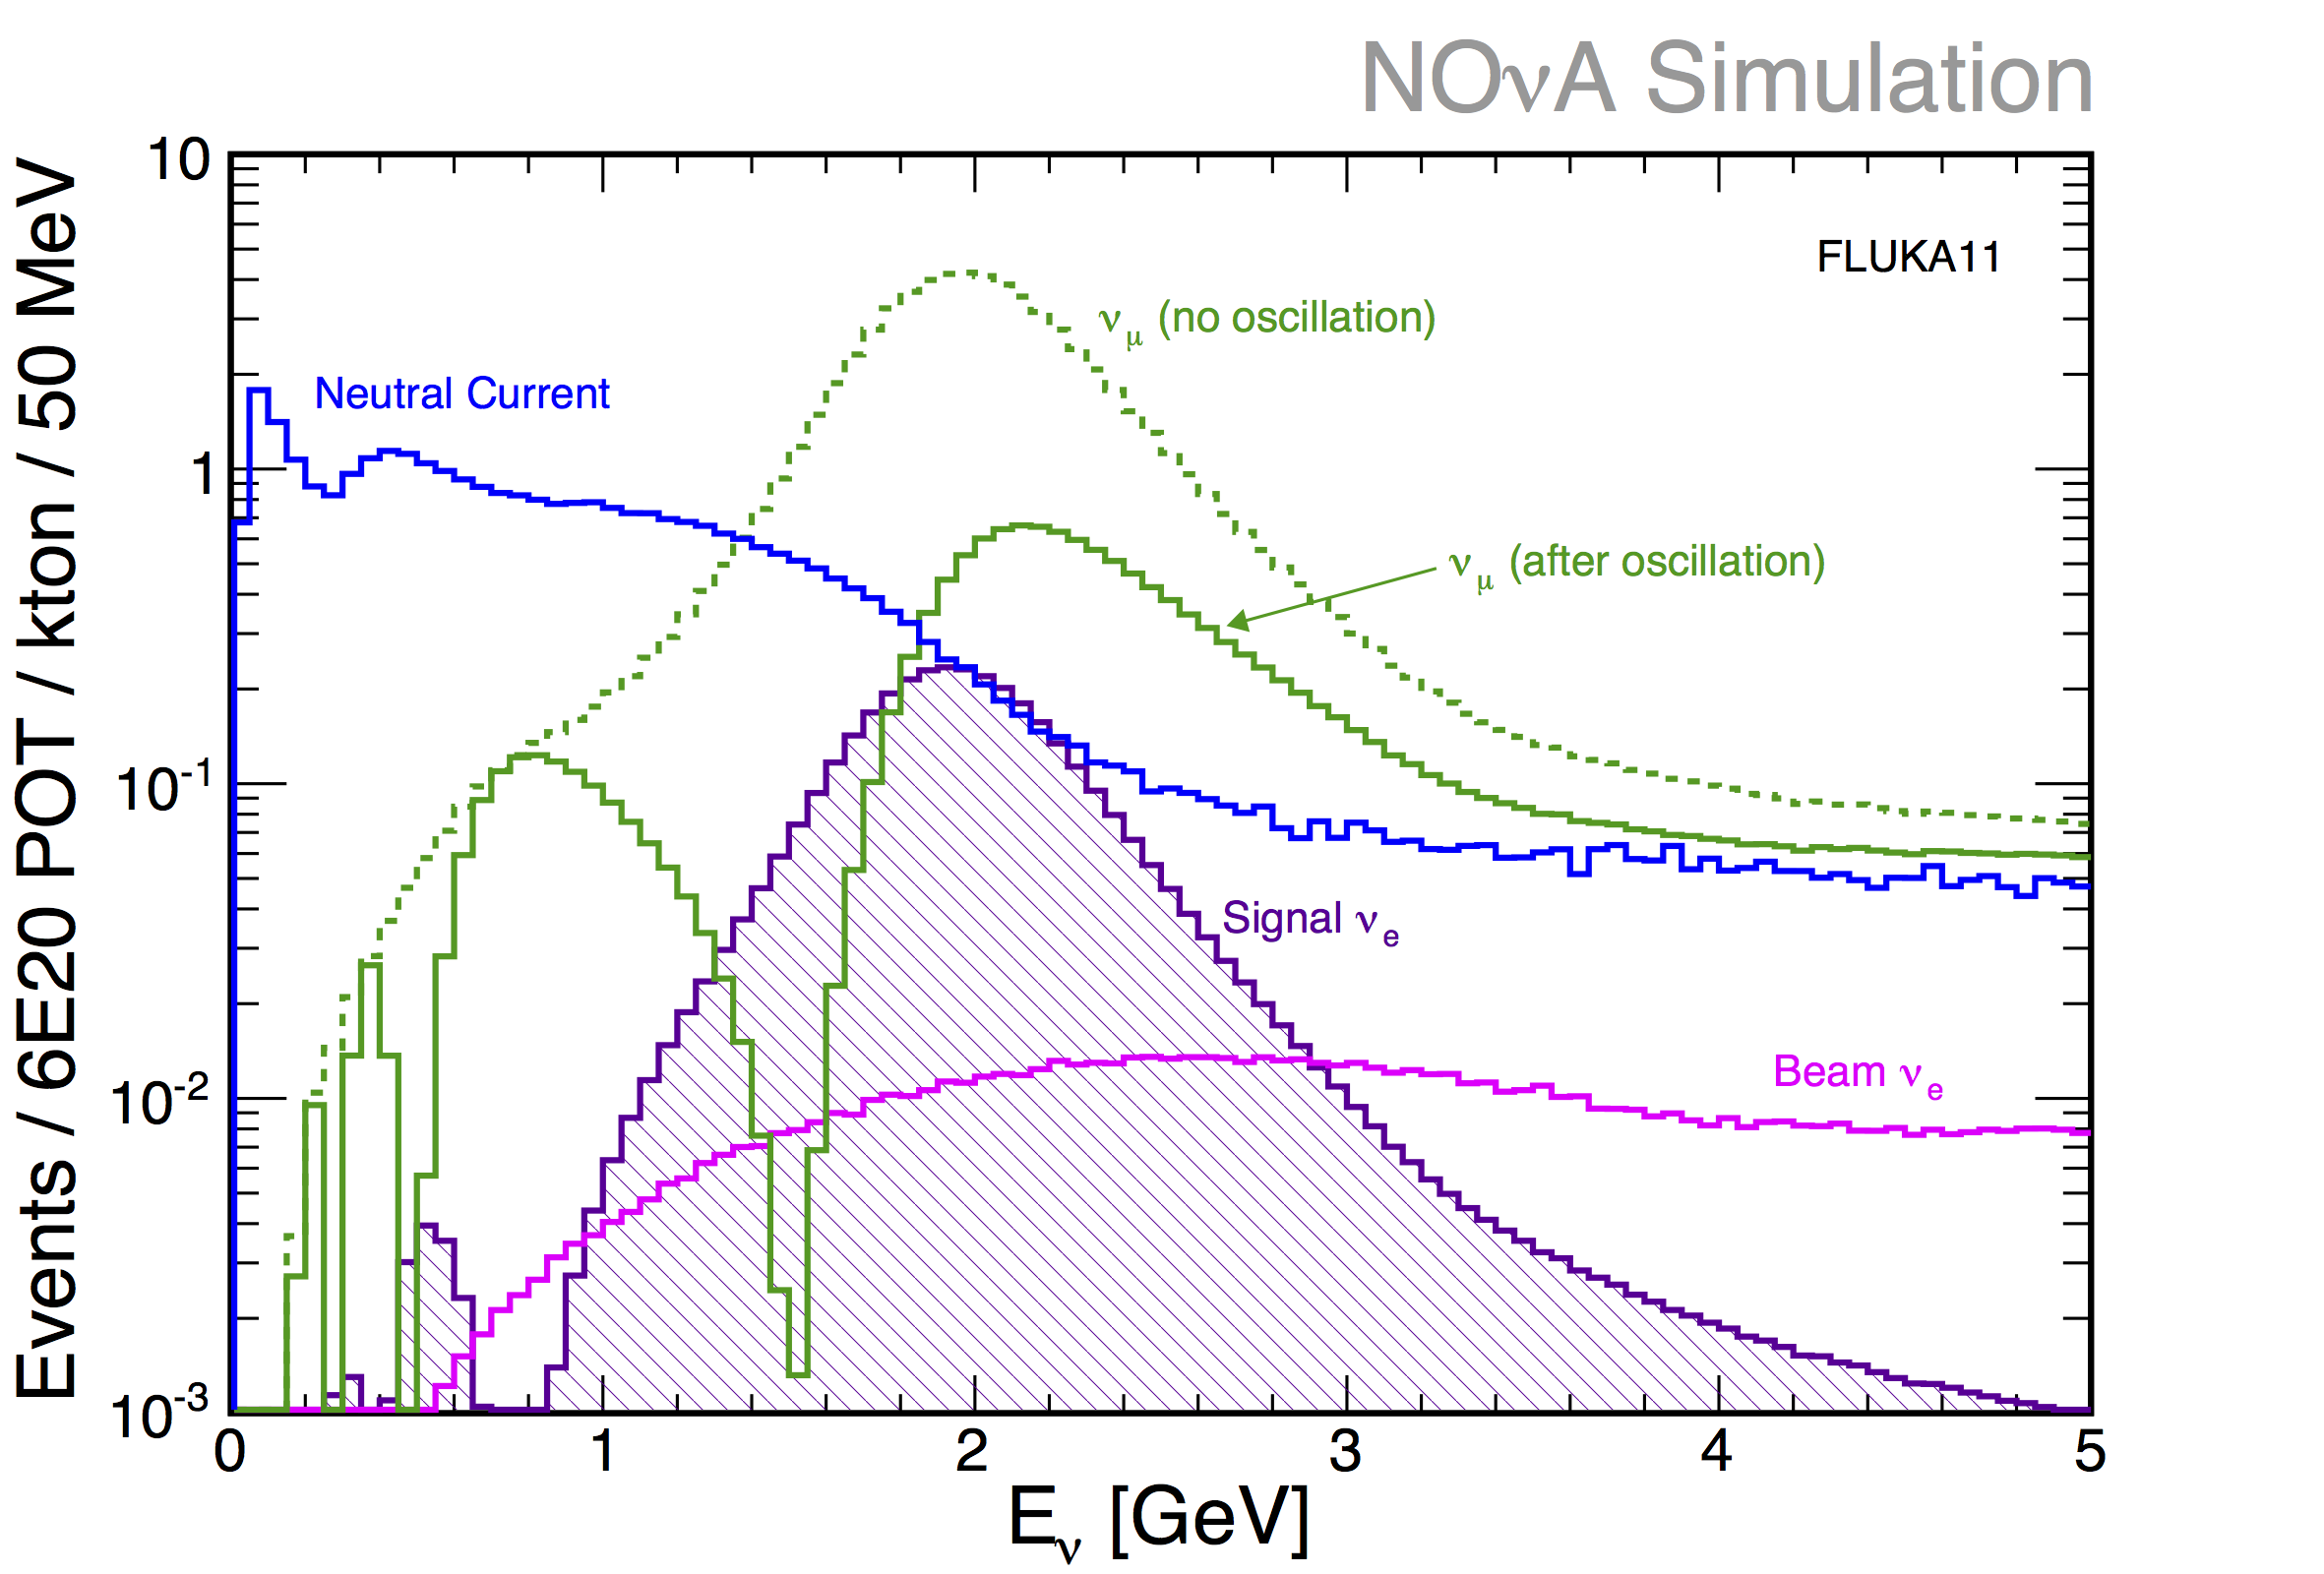
\includegraphics[width=.47\textwidth]{figures/BeamFluxXSec.png} \\
  \end{tabular}
  \caption[Probability of $\nue$ Appearance and Expected Event Rates for \nova]{Left: the probability of $\nue$ appearance. The probabilities are calculated assuming standard three flavor oscillations using the relevant values shown in table \ref{tab:LOverEValues}, except for $\delta_{CP}$ which is here set to $3\pi/2$. Right: The expected number of events as a function of true neutrino energy (with the exception of NCs), for individual components. The NC component is shown as a function of true visible energy $E_{vis} \equiv E_\nu \times y_{Bj}$, where $y_{Bj}$ is the fractional energy loss Bjorken scaling variable.}
  \label{fig:PMuEFluxXSec}
\end{figure}

As with the main \nova~analyses, the off-axis nature of the experiment has both pros and cons when searching for sterile oscillations via NC disappearance. Obviously a reduced neutrino flux is not great when searching for neutrino interactions. However, the CC backgrounds are highly suppressed due to oscillations, even with the $\nue$ appearance. This makes the selection of a relatively pure sample of NC events at the FD a much easier task.

\section{The \nova~Detectors}
